% Alter some LaTeX defaults for better treatment of figures:
    % See p.105 of "TeX Unbound" for suggested values.
    % See pp. 199-200 of Lamport's "LaTeX" book for details.
    %   General parameters, for ALL pages:
    %\renewcommand{\topfraction}{0.9}	% max fraction of floats at top
    %\renewcommand{\bottomfraction}{0.8}	% max fraction of floats at bottom
    %   Parameters for TEXT pages (not float pages):
    %\setcounter{topnumber}{2}
    %\setcounter{bottomnumber}{2}
    %\setcounter{totalnumber}{4}     % 2 may work better
    %\setcounter{dbltopnumber}{2}    % for 2-column pages
    %\renewcommand{\dbltopfraction}{0.9}	% fit big float above 2-col. text
    %\renewcommand{\textfraction}{0.07}	% allow minimal text w. figs
    %   Parameters for FLOAT pages (not text pages):
    %\renewcommand{\floatpagefraction}{0.7}	% require fuller float pages
	% N.B.: floatpagefraction MUST be less than topfraction !!
    %\renewcommand{\dblfloatpagefraction}{0.7}	% require fuller float pages

\documentclass[a4paper,12pt,titlepage]{book}
\usepackage{palatino}
\usepackage{xtab}
\usepackage{subfig}
\usepackage{graphicx}
\setkeys{Gin}{width=5.7cm} % default image width
%\usepackage[section]{placeins}
\usepackage{hyperref}
\usepackage{microtype}
\graphicspath{{images/}}

\renewcommand*\sfdefault{ugq}
\newcommand{\lsdjversion}{v7.9.0}

\author{Copyright \copyright~Johan Kotlinski \thanks{Aaron U made minor contributions. Thanks!}}
\title{Little Sound Dj \lsdjversion{}}


\hypersetup{breaklinks=true,
colorlinks=true,
pdfauthor=Johan Kotlinski,
pdftitle=Little Sound Dj \lsdjversion{}}

\begin{document}

\begin{titlepage}
\begin{center}
\vspace*{2.75cm}
\includegraphics[width=9.85cm]{lsdj_black_rgb}\\
\vspace*{1.00cm}
\normalfont\sffamily
\LARGE
Little Sound Dj \lsdjversion{}
\\
%\LARGE Little Sound Dj \lsdjversion{}\\
\vspace*{0.65cm}
Operating Manual
\end{center}
\end{titlepage}

\maketitle
\tableofcontents
\chapter{Introduction}
\section{Hi!}
First of all, thanks for trying out Little Sound Dj!

A lot of effort has been put into making this program as powerful and fast-worked
as possible. If you don't have previous experience from similar ``tracker"-like
music editors, the amount of new concepts may seem a bit overwhelming at first.
Please, try not to stress about it. Learn step by step, keep it fun and progress
at your own pace. Within an hour or two, you should know enough about the
program to make your own first songs.

This manual is mostly written as an absolute beginners' guide, but it also serves as a reference
that covers everything in the program. However, there still
is a lot of information that would not fit into a manual like this. I highly recommend
checking out the user-maintained Wiki site at \url{http://wiki.littlesounddj.com} -
it contains material like tutorials, tips and tricks, and
hardware-related DIY projects. Also, the Facebook group
at \url{https://www.facebook.com/groups/LittleSoundDJ/} is useful for getting in touch
with other users.
If you have questions or bug reports, please e-mail
\href{mailto:info@littlesounddj.com}{info@littlesounddj.com}.

Happy tracking!

\textit{/Johan}

\section{Important Notice}

Turning off the Game Boy while playing may cause your songs to be lost, so please avoid that.
Also, it is best to avoid using the program when batteries are low because the Game Boy can risk shutting down without warning.
Low battery level is indicated by the red light on your Game Boy
becoming faint, or the screen becoming dim.

\section{Game Boy Sound}
The Game Boy sound chip has four channels, each with 4-bit audio resolution.

\begin{description}
\item[Pulse Channel 1] Square wave with envelope and sweep functions.
\item[Pulse Channel 2] Square wave with envelope function.
\item[Wave Channel] Soft synthesizer, sample playback and speech synthesis.
\item[Noise Channel] Noise with envelope and shape functions.
\end{description}


\section{Key Presses}
In this documentation, key presses are marked up in this fashion:
\begin{description}
\item[\textsc{a}] \textsc{a} button
\item[\textsc{b}] \textsc{b} button
\item[\textsc{start}] start button
\item[\textsc{select}] select button
\item[\textsc{left}] left arrow
\item[\textsc{right}] right arrow
\item[\textsc{up}] up arrow
\item[\textsc{down}] down arrow
\item[\textsc{cursor}] pressing any arrow key
\item[\textsc{left/right}] pressing left or right arrow
\item[\textsc{up/down}] pressing up or down arrow
\item[\textsc{select+a}] pressing \textsc{a} while holding \textsc{select}
\item[\textsc{select+(b,b)}] pressing \textsc{b} twice, while holding \textsc{select}
\end{description}

\section{Navigating the Program}
After starting up LSDj, you should be facing a screen like the one in figure~\ref{fig:song}.

\begin{figure}[hbtp]
\centering
\fbox{ \includegraphics{song} }
\caption{Song Screen}
\label{fig:song}
\end{figure}

The \textsc{song} title at the top left of the window indicates that this is the song screen, the
window where you arrange your songs. The four columns with dashes each represent a
Game Boy sound channel. There are two pulse wave channels, one custom wave channel
(which uses sampled drum kits or soft-synthesized wave forms), and one noise channel. You
can move around between the different channels using the cursor key.
\begin{figure}[hbtp]
\centering
\fbox{ \includegraphics{map} }
\caption{Screen Map}
\label{fig:map}
\end{figure}

Little Sound Dj uses several screens, which are laid out on a \begin{math} 5 \times 3 \end{math} map, displayed in the
bottom right of the screen (figure~\ref{fig:map}). The most useful screens are laid out in the middle row, also called
the main row. It contains the song, chain, phrase, instrument and table screens. These screens
are ordered after level detail. The leftmost song screen presents an overview over the entire
song, whereas the rightmost table screen is for detailed instrument programming. You can
navigate between the different screens by holding \textsc{select} and pressing the cursor key.

The song, chain and phrase screens are used for sequencing, and work together in a tree-structure
fashion. The phrase screen is a 16-step sequencer where the actual note data is
entered. The chain screen is a 16-step sequencer where you can enter sequences of phrases to
be played back. The song screen is a 256 step long sequencer, where you enter sequences of
chains to be played back.

\section{Making Your First Sounds}
Navigate to the song screen, and put the cursor on the \textsc{pu1} column. Now tap the \textsc{a} button
to insert a new chain. The digit 00 should appear at the cursor. You can now edit chain 0 by pressing \textsc{select+right} and entering the chain screen. There, go through the
same procedure: tap \textsc{a} to insert a new phrase, and press \textsc{select+right} to go to the
phrase screen.

\begin{figure}[hbtp]
\centering
\fbox{\includegraphics{phrase}}
\caption{Phrase Screen}
\label{fig:phrase1}
\end{figure}

In the phrase screen, you can enter notes to be played back. Move the cursor to the note
column and press \textsc{a} to enter a note. The text \textsc{c 2} will appear: C being the note, and 2 being the
octave. Press \textsc{start} to play back the phrase. Note how the phrase is played back from the
top of the screen to the bottom. You can change the note value by holding \textsc{a} and pressing the
cursor button. \textsc{a+left/right} changes the note, and \textsc{a+up/down} changes octave.

You can now try to move the cursor up and down and insert more notes in other positions. If
you want to delete a note, hold \textsc{b} and press \textsc{a}. When you have finished listening, press
\textsc{start} again to stop the phrase.

The clean pulse sound might get a bit dull after while. Let's move on to the instrument
screen by pressing \textsc{select+right}.

\begin{figure}[hbtp]
\centering
\fbox{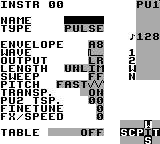
\includegraphics{instr-pulse}}
\caption{Instrument Screen}
\label{fig:instr}
\end{figure}

In the instrument screen, we can make the sound a little bit more interesting. Try to change
the envelope and wave fields by moving the cursor there and pressing \textsc{a+left/right}. Try
to modify the envelope setting from \texttt{A8} to \texttt{A3}. Now, press \textsc{start} again to hear any
change in sound. The sound should now be more bouncy.

The type field sets the instrument type. The instrument types are specific to each sound channel -- pulse instruments should only be played back in the pulse channels, wave and kit
instruments in the wave channel, and noise instruments in the noise channel.

Let's try out the sampled drum kits. Now, we have to change the channel to the wave channel.
Go back to the song screen, move the cursor over to the wave channel, and create a new
chain and a new phrase the way you did before (tapping \textsc{a} on empty steps). 
Then tap \textsc{a} in the note column, and automatically a new instrument is created. 
Press \textsc{select+right} to edit that instrument, change the instrument type to 
\textsc{kit} by pressing \textsc{a+right} once on the type field, then go back to 
the phrase screen. Now, you should be able to enter drum sounds the same way you entered notes before.

\section{Initial Troubleshooting}

Does Little Sound Dj behave strangely? Here are some things to try:

\begin{itemize}
\item If your cartridge doesn't start up at all, and only shows a garbled Nintendo logo at startup, the problem might be oxide on the cartridge pins. Try removing and re-inserting your cartridge about thirty to forty times. You can also clean the cartridge pins using a cotton swab dipped in isopropyl alcohol.
\item If the software starts to act up, it might be worth doing a full reset of the cartridge memory. This is done by navigating to the project screen and pressing \textsc{select+a+b} on the \textsc{load/save file} button.
\item Search for more help on the Little Sound Dj Wiki (\url{http://wiki.littlesounddj.com}) or ask in the Facebook group.
\end{itemize}

\section{Hexadecimal Number System}

Before moving on to the next chapter, now is a good time to get introduced to the hexadecimal number system that Little Sound Dj uses for representing values.

The hexadecimal number system works the same way as the traditional decimal number system. The only difference is that its base is 16 instead of 10. This means it consists of 16 unique symbols: the digits 0 to 9, followed by the letters A to F. For clarity, this manual will mark hexadecimal values with a dollar sign.
As an example, let's print a table of numbers -- first with decimal digits, then with
hexadecimal digits\ldots

\begin{figure}[hbtp]
\centering

\begin{tabular}{r|r|r|r|r|r|r|r|r|r|r}
 Decimal & 1 & 2 & 3 & 4 & 5 & 6 & 7 & 8 & 9 & 10 \\
\hline
 Hexadecimal & \$1 & \$2 & \$3 & \$4 & \$5 & \$6 & \$7 & \$8 & \$9 & \$A \\
\end{tabular}

\begin{tabular}{r|r|r|r|r|r|r|r|r|r|r}
 Decimal & 11 & 12 & 13 & 14 & 15 & 16 & 17 & 18 & 19 & 20 \\
\hline
 Hexadecimal & \$B & \$C & \$D & \$E & \$F & \$10 & \$11 & \$12 & \$13 & \$14  \\
\end{tabular}

\end{figure}

Note that the hexadecimal and decimal values are really equal; just the representations differ.
The reason to use the hexadecimal system here is to save screen space; with hexadecimal
numbers, it is possible to represent every byte value using no more than two digits. (The
value range is 0 to 255 -- that is, \$0 to \$FF.)

Representing negative numbers with two digits only can be a problem. In Little Sound Dj,
the numbers values wrap around. That means, when subtracting one from the smallest possible
number (\$0), it will jump to the highest possible value (\$FF). So \$FF can represent -1 as well as 255, depending on the situation.

If you don't get all this immediately -- please don't worry too much -- it will become clear to you as you spend time with the program.




\chapter{The Screens}
As stated before, Little Sound Dj has several screens, laid out in a screen map of size \begin{math} 5 \times 3 \end{math}. You can
navigate between the screens by pressing \textsc{select+cursor}.
\section{Screen Map}
\begin{figure}[htbp]
\centering
\begin{tabular}{|c|c|c|c|c|l}

	\cline{0-4}
	\multicolumn{3}{|c|}{ } & &
	\\
	\multicolumn{3}{|c|}{Project} & Wave &
	\\
	\multicolumn{3}{|c|}{ } & &
	\\
	\cline{0-3}
	& & & & & \\
	Song & Chain & Phrase & Instr. & Table  & \begin{math} \leftarrow \end{math} Main Row \\
	& & & & & \\
	\cline{0-4}
	\multicolumn{3}{|c|}{} & &
	\\
	\multicolumn{3}{|c|}{Groove} & Synth & Groove
	\\
	\multicolumn{3}{|c|}{} & &
	\\
	\cline{0-4}
\end{tabular}
%\caption{Screen Map.}
\end{figure}

The song, chain and phrase screens are used for sequencing and arranging. The wave, synth,
instrument and table screens are used for sound programming. \footnote{There are also three hidden
screens, not shown on the map: The file, word and help screens. We will come back to these later.}

The remaining screens, project and groove, have more general purposes. The bulk of your activities will however probably be in the so-called "main row," in the middle of the map, as that's where the composing is done.

\section{Starting and Stopping}

When pressing \textsc{start} in the song screen, Little Sound Dj will always try to play all four
channels. When pressing \textsc{start} in the other screens, Little Sound Dj will only try to play the
channel that's indicated in the three-letter field at the right edge of the screen (\textsc{pu1}, \textsc{pu2}, \textsc{wav} or \textsc{noi}).

If you want to start playing all four channels from some other screen than the song screen,
you can do that by pressing \textsc{select+start}.

\section{Song Screen}

\begin{figure}[hbtp]
\centering
\fbox{ \includegraphics{song} }
\caption{Song Screen}
%\label{fig:song}
\end{figure}

The song screen
%(figure~\ref{fig:song})
is the highest level of the sequencer. This is where you arrange your songs.

The screen contains four columns, one for each channel. The columns contain lists of chains, which will be played in order from top to bottom. Different chains are used for different channels.

To insert a chain, move the cursor to an empty step and press \textsc{a}. If you want to add a new
chain, press \textsc{a} twice. To edit a chain, move the cursor to the chain number and press
\textsc{select+right}. To remove a chain, press \textsc{b+a}.

To start or stop playing all channels in the song screen, press \textsc{start}. To instantly re-start all channels in the song screen, press \textsc{select+start} (this has the same effect as pressing \textsc{start, start} quickly).

\includegraphics[width=1cm]{tip}TIP!
\begin{itemize}
\item \textit{Pressing \textsc{b+a} on an empty step moves the chains below it upwards.}
\item \textit{\textsc{b+up/down} navigates up/down by \$10 rows.}
\item \textit{You can add or remove song screen bookmarks by tapping \textsc{b} three times \textsc{(b, b, b)}. This will shade the area under the cursor.}
%	\marginpar{\includegraphics[width=1cm]{tip}TIP!}
\end{itemize}

The number of rows in the song screen is limited to 255 (\$00-\$FE).

\section{Chain Screen}
Chains are used for stringing phrases together, thus creating a unit composed of multiple
phrases. A chain can represent a longer block of rhythm, such as a melody or a bass-line.

The chain screen contains two columns. The first column contains the list of phrases that are
to be strung together, while the second column transposes the phrase on that row.

\begin{figure}[hbtp]
\centering
\fbox{ \includegraphics{chainexample} }
\caption{Chain Screen}
\label{fig:chainexample}
\end{figure}

Example:
The chain in figure~\ref{fig:chainexample} would play phrase 3, adding 5 semitones to each note, and then play each of the phrases 4, 5, 6, without transposing.

To add a phrase to the chain, move the cursor to an empty step and press \textsc{a}. If you want to
insert a new phrase, press \textsc{a} twice. To edit a phrase, move the cursor to the phrase number
and press \textsc{select+right}.

When editing a chain, you can go to the chain in a neighboring channel by pressing \textsc{b+left/right}. It is also possible to go to the next or previous chain in the song screen by
pressing \textsc{b+up/down}.

The different channels all share the same set of chains; that is, no chain is ever assigned to a
specific channel. The number of chains is limited to 128 (\$00-\$7F).

\section{Phrase Screen}

\begin{figure}[hbtp]
\centering
\fbox{ \includegraphics{phrase} }
%\caption{Phrase Screen}
%\label{fig:phrase}
\end{figure}

The phrase screen is the most fundamental part of the sequencer; this is where you enter the actual note data. The phrase screen has four columns: the note column, the instrument column, and the command and command value columns.

Like chains, phrases may be played on any channel. A phrase might however sound very different depending on the channel it is played back on. Example: If you have programmed a phrase to play a melody using a pulse instrument, that phrase can be played back in either of the pulse channels with good results, but it usually doesn't make sense to play back the phrase in the wave or noise channels.

The note column may look different depending on which instrument type is used. Most instruments show the note followed by the octave. However, instruments that play back samples (\textsc{kit}, \textsc{speech}) show the sample or word names instead.

The instrument column is used for selecting instruments. In total, you can use 64 different instruments, editable in the instrument screen.

\includegraphics[width=1cm]{tip}TIP!
\begin{itemize}
\item \textit{It is possible to change the pitch without retrigging the instrument by leaving the instrument column empty. 
You can remove the instrument number by pressing \textsc{B+A} in the instrument column.}
%	\marginpar{\includegraphics[width=1cm]{tip}TIP!}
\end{itemize}

The command column can be used to add effects to your phrase. For example, the K command kills the sound on the channel.

The number of phrases is limited to 255 (\$00-\$FE). The number of the phrase that is being edited is displayed in the top left corner of the screen.

\includegraphics[width=1cm]{tip}TIP!
\begin{itemize}
\item \textit{All phrases are 16 steps long by default, but it is also possible to set a shorter length by using the H (hop) command. 
Placing H00 ends the phrase at the line before it is placed.}
%	\marginpar{\includegraphics[width=1cm]{tip}TIP!}
\end{itemize}


\section{Instrument Screen}

\begin{figure}[hbtp]
\centering
\fbox{ 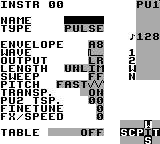
\includegraphics{instr-pulse} }
\caption{Instrument Screen}
\label{fig:instr2}
\end{figure}

There are five types of instruments available:

\begin{description}
\item[\textsc{pulse}] This instrument type produces pulse waves, and is used in pulse channels 1 and 2.
\item[\textsc{wave}] This instrument type can play back waves synthesized using the synth screen. It is used in the wave channel.
\item[\textsc{kit}] This instrument type plays sampled kits, stored in \textsc{rom}. (The samples are stored in 4-bit 11,468 Hz audio.) It is used in the wave channel.
\item[\textsc{noise}] This instrument type produces filtered noise, and is used in the noise channel.
\item[\textsc{speech}] This instrument is locked to instrument number \$40, and is used for programming speech. For learning how to generate speech, please read chapter \ref{speech-chapter}.
\end{description}

You can change the instrument type by going to the type row and pressing \textsc{a+cursor}.

Remember that instruments don't automatically play in the right channel. For example, if you want to use a kit instrument to play drum samples, you have to do the following:

\begin{enumerate}
\item Go to the song screen, move cursor to the wave column, and insert a new chain by tapping \textsc{a}.
\item	Edit the chain by pressing \textsc{select+right}.
\item	Insert a new phrase by tapping \textsc{a}.
\item	Edit the phrase by pressing \textsc{select+right}. Now, you have a new phrase that is mapped to the wave channel.
\item	Create a new instrument by moving the cursor to the instrument column and tapping \textsc{a}.
\item	Press \textsc{select+right} to edit the instrument.
\item	Change the instrument type to \textsc{kit}.
\item	Go back to the phrase screen to start using your new instrument.
\end{enumerate}

\includegraphics[width=1cm]{tip}TIP!
\begin{itemize}
	\item \textit{In the instrument screen, press \textsc{select+b} to copy instruments and \textsc{select+a} to paste.}
%\marginpar{\includegraphics[width=1cm]{tip}TIP!}
\end{itemize}

\subsection{General Instrument Parameters}
\label{general-instrument-parameters}

These parameters are used in most instrument types.

\begin{description}
	\item[\textsc{name}] Name the instrument by pressing \textsc{a}. This is useful for keeping track of your instruments. The instrument name will also be shown in the border when selecting instruments in the phrase screen.
	\item[\textsc{type}] Use this to specify the instrument type.
	\item[\textsc{length}] Change the sound length.
	\item[\textsc{pan}] Pan the sound to left/right/both/none speakers. (Use the headphone output to hear the difference!)
    \item[\textsc{pitch}] Controls the behavior of \textsc{p}, \textsc{l} and \textsc{v} commands. \textsc{A+u/d} switches pitch update speed: \textsc{fast} updates pitch at 360 Hz; \textsc{tick} updates pitch every tick; \textsc{step} is like \textsc{fast} except that \textsc{p} changes the pitch only once instead of sliding; \textsc{drum} is like \textsc{fast} with logarithmic pitch, useful for \textsc{p} kicks. \textsc{A+l/r} changes vibrato shape between downwards triangle, saw and square, and upwards triangle, saw and square.
    \item[\textsc{transp.}] When \textsc{on}, the pitch will be affected by project and table transposes. Turning transpose \textsc{off} is useful for kick drums, for example.
	\item[\textsc{fx/speed}] Controls the rate of C and R commands, as well as P and V commands when pitch is set to \textsc{tick}. (P commands in the noise channel are also affected.) \textsc{fx/speed} value of 0 is the fastest rate, while \$F is the slowest.
    \item[\textsc{table}] Selects a table to run when a note is played. If you want to edit the table, press \textsc{select+right} to go to the table screen. To create a new table, press \textsc{a,a}. To clone the table, press \textsc{select+(b,a)}. By default table is set to \textsc{play} however, pressing \textsc{A+//r} toggles the table to \textsc{step}. This option extends the table functionality. When \textsc{step} is activated, Little Sound Dj advances through the table one step each time the instrument is triggered.
\end{description}

\subsection{Pulse Instrument Parameters}
\label{detune}

\begin{figure}[htpb]
	\begin{center}
\fbox{ 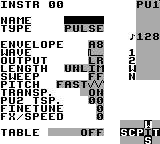
\includegraphics{instr-pulse} }
	\end{center}
	\caption{Pulse Instrument Screen}
	\label{fig:instr-pulse}
\end{figure}

\begin{description}
	\item[\textsc{envelope}] The first digit sets initial amplitude (0-\$F); the second digit sets release (0, 8: none, 1-7: decrease amplitude, 9-\$F: increase amplitude).
	\item[\textsc{wave}] Choose the wave type to be used.
	\item[\textsc{sweep}] Modulate the frequency. This only works on pulse channel 1. See Sweep/Shape (\textsc{s}) command documentation for further information.
\end{description}

The detune settings can be used to create interesting phase effects, when the same phrase is played on both pulse channels:

\begin{description}
	\item[\textsc{pu2 tsp}] Transpose pulse channel 2 in semitones.
	\item[\textsc{finetune}] Detune pulse channel 1 downwards, channel 2 upwards.
\end{description}

\subsection{Wave Instrument Parameters}

The wave instrument can play back synth sounds generated by the soft synthesizer found in the \textsc{synth} screen.

\begin{figure}[hbtp]
	\begin{center}
		\fbox { 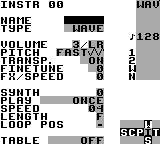
\includegraphics{instr-wave} }
	\end{center}
	\caption{Wave Instrument Screen}
	\label{fig:instr-wave}
\end{figure}

\begin{description}
	\item[\textsc{volume}] Set amplitude (0=0\%, 1=25\%, 2=50\%, 3=100\%) and pan
	\item[\textsc{finetune}] Detune the synth by +\/-0-\$F
	\item[\textsc{synth}] Select the synth sound to play back. To edit the synth sound being used, press \textsc{select+down} to go to the \textsc{synth} screen. If you want to use a new synth, tap \textsc{a} twice. If you want to clone the current synth to a new synth, press \textsc{select+b,a}.
	\item[\textsc{play}] How to play back the synth sound: Once, loop, pingpong loop or manual. By selecting manual, only the first wave in the synth sound will be played, allowing you to select waves manually using the \textsc{f} command.
	\item[\textsc{speed}] Set how fast the synth sound should be played back.
	\item[\textsc{length}] Set the length of the synth sound.\footnotemark
\footnotetext{For each length value, the following waves are played:
\begin{center}
\begin{tabular}{ |c|l| } 
 \hline
Length & Wave Frames \\ \hline
0 & 0 \\ \hline
1 & 0, \$F \\ \hline
2 & 0, 7, \$F \\ \hline
3 & 0, 5, \$A, \$F \\ \hline
4 & 0, 3, 7, \$B, \$F \\ \hline
5 & 0, 3, 6, 9, \$C, \$F \\ \hline
6 & 0, 2, 5, 7, \$A, \$D, \$F \\ \hline
7 & 0, 2, 4, 6, 9, \$B, \$D, \$F \\ \hline
8 & 0, 1, 3, 5, 7, 9, \$B, \$D, \$F \\ \hline
9 & 0, 1, 3, 5, 7, 8, 9, \$B, \$D, \$F \\ \hline
\$A & 0, 1, 3, 4, 6, 7, 9, \$B, \$C, \$E, \$F \\ \hline
\$B & 0, 1, 2, 4, 5, 7, 8, \$A, \$B, \$D, \$E, \$F \\ \hline
\$C & 0, 1, 2, 3, 5, 6, 7, 9, \$A, \$B, \$D, \$E, \$F \\ \hline
\$D & 0, 1, 2, 3, 4, 6, 7, 8, 9, \$B, \$C, \$D, \$E, \$F \\ \hline
\$E & 0, 1, 2, 3, 4, 5, 6, 7, 9, \$A, \$B, \$C, \$D, \$E, \$F \\ \hline
\$F & 0, 1, 2, 3, 4, 5, 6, 7, 8, 9, \$A, \$B, \$C, \$D, \$E, \$F \\ \hline
\end{tabular}
\end{center}
}
	\item[\textsc{loop}] Set the loop point of the synth sound.
\end{description}

\subsection{Kit Instrument Parameters}

\begin{figure}[hbtp]
	\begin{center}
	\fbox {	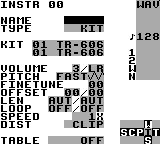
\includegraphics{instr-kit} }
	\end{center}
	\caption{Kit Instrument Screen}
	\label{fig:instr-kit}
\end{figure}

\begin{description}
	\item[\textsc{kit}] Choose the kits to use. The first kit will be used in the left note column in the phrase screen; the second kit will be used in the right note column in the phrase screen.
	\item[\textsc{finetune}] Pitch shift.
	\item[\textsc{offset}] Set the start loop point. If \textsc{loop} is set to \textsc{off}, this value can be used for skipping the initial part of a sound.
	\item[\textsc{len}] Set the sound length. (\textsc{aut}=always play the sample to its end.)
	\item[\textsc{loop}] Loop the sample. (\textsc{off}=don't loop, \textsc{on}=loop sound and start playing from custom offset, \textsc{atk}=loop sample and start playing from the beginning.)
	\item[\textsc{speed}] Play the sample at full speed or half speed.
	\item[\textsc{dist}] Select the algorithm that should be used when two kits are mixed together. \textsc{clip} is the default type. \textsc{shape} and \textsc{shape2} sound similar to \textsc{clip}, but with more high frequencies and less bass. \textsc{wrap} can be used to add some interesting digital distortion. When pressing \textsc{a+(left, left)} while \textsc{clip} value is selected, the program will jump out of range and play back sound from raw memory when clipping.
\end{description}

\includegraphics[width=1cm]{tip}TIP!
\begin{itemize}
	\item \textit{For those running LSDj on emulator or with backup gear, there is a Java application for replacing the original sample kits available at} \url{https://github.com/Eiyeron/lsdpatch/releases}.
\end{itemize}

\subsection{Noise Instrument Parameters}
\label{noise-instrument-parameters}

\begin{figure}[htpb]
	\begin{center}
		\fbox { 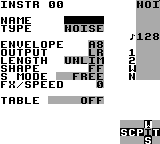
\includegraphics{instr-noise} }
	\end{center}
	\caption{Noise Instrument Screen}
	\label{fig:instr-noise}
\end{figure}

\begin{description}
	\item[\textsc{envelope}] First digit is initial amplitude (0-\$F); second digit is release (0, 8: none, 1-7: decrease amplitude, 9-\$F: increase amplitude).
    \item[\textsc{shape}] Noise generator control. The first digit changes pitch by octave, the second digit divides the frequency. Set the second digit to 0-7 for periodic noise, 8-\$F for random noise.
        For an in-depth technical explanation, refer to \href{https://google.com\&q=gbsound.txt}{gbsound.txt}.
	\item[\textsc{s cmd}] When set to \textsc{free}, S commands may randomly\footnotemark mute the sound when changing noise shape. When set to \textsc{stable}, S commands are limited so that sound will never be muted by accident. This will restrict the shape of the instrument to either periodic noise (if the second digit of shape is 0-7) or random noise (if the second digit of shape is 8-\$F) only.
\footnotetext{There is a 1 in 256 chance (0.4\%) that the sound gets muted when a shape that ends with digit 8-\$F
        is changed so that it ends with digit 0-7.}
\end{description}

\subsection{Speech Instrument Parameters}

For information about how to generate speech, please read chapter \ref{speech-chapter}.

The number of instruments is limited to 64 (hexadecimal: \$00-\$39).

\section{Table Screen}

Tables are sequences of transposes, commands and amplitude changes which can be executed at any speed and applied to any channel. By setting a table in the instrument screen, the table will start every time you play the instrument. This allows you to create more interesting sounds than would be possible using the instrument screen alone.

Tables contain six columns. The first column is the envelope column, used to create custom amplitude envelopes. Next is the transpose column, used to transpose the played note by a number of semitones. The other columns are command columns like the one in the phrase screen.

The default table speed of one tick per step can be changed using the G command.

\includegraphics[width=1cm]{tip}TIP!
\begin{itemize}
	\item \textit{The transpose column has special functionality when using \textsc{kit} or \textsc{noise} type instruments. For \textsc{kit}, the transpose column works as a pitch shifter. For \textsc{noise}, the transpose column works like the \textsc{s} (shape) command.}
\end{itemize}

\subsection{Custom Envelope Example}

The first digit in the envelope column sets the amplitude; the second digit sets for how many ticks that amplitude should remain (0-\$E). Setting the second digit to \$F hops to the row number of the first digit.

\begin{figure}[htpb]
	\begin{center}
		\fbox{		\includegraphics{table-amp} }
	\end{center}
	\caption{Table Envelope Example}
	\label{fig:table-amp}
\end{figure}

The table in figure~\ref{fig:table-amp} creates an amplitude envelope with short attack and medium sustain. It could be used for a bass instrument.

\subsection{Arpeggio Example}

\begin{figure}[htpb]
	\begin{center}
		\fbox{ \includegraphics{table-arp}}
	\end{center}
	\caption{Arpeggio Example}
	\label{fig:table-arp}
\end{figure}

A typical use for tables is to create arpeggios. This is a musical term for playing notes very fast, so that the listener will get the impression that a chord is played. The table in figure~\ref{fig:table-arp} would emulate striking a major chord.

Shorter arpeggios can just as well be created using the C (chord) command in phrases (see \ref{command-chord} for example). Tables however still have to be used for creating longer arpeggios.

To view different tables, press \textsc{b+cursor}.

\includegraphics[width=1cm]{tip}TIP!
\begin{itemize}
	\item \textit{To give an instrument some attack, transpose the first table row a few steps up or down.}
	\item \textit{There is a shortcut between the phrase and table screens. Press \textsc{select+right} on an A command in the phrase screen to edit the table selected with the A command. To jump back, press \textsc{select+left}.}
\end{itemize}

The number of tables is limited to 32 (\$00-\$1F).

\section{Groove Screen}

Grooves define the speed by which your phrases and tables are played back. They can be used for giving your songs some extra swing. The different sound channels do not need to be synchronized to each other; this means that you can use a separate groove for each phrase and table.

\begin{figure}[htbp]
	\begin{center}
		\fbox{ \includegraphics{groove} }
	\end{center}
	\caption{Groove Screen}
	\label{fig:groove}
\end{figure}

To understand grooves, you need to know that the sequencer's time handling is based on an abstract time period called \emph{tick}. The length of a tick varies with the song tempo; at 128 BPM, a tick is approximately 1/50th of a second. In the groove screen, you can specify how many ticks each note step should be played.
The groove in figure~\ref{fig:groove} would make the sequencer spend approximately 6/50th of a second on every note step.

\begin{figure}[htbp]
	\begin{center}
		\fbox{ \includegraphics{groove-swing} }
	\end{center}
	\caption{Swing Example}
	\label{fig:groove-swing}
\end{figure}

You can also use the groove screen to create custom rhythms. The groove in figure~\ref{fig:groove-swing} would make the sequencer spend 8/50th of a second on even note steps, and 5/50th of a second on odd note steps, creating a swing. With thoughtful programming, grooves can also be used to create triplets and other complex rhythm structures.

Groove 0 is the default groove for all phrases. If you want to, you can easily switch to another groove using the groove (\textsc{g}) command in the phrase screen.

You can select the groove you wish to edit by pressing \textsc{b+cursor}.

\includegraphics[width=1cm]{tip}TIP!
\begin{itemize}
	\item \textit{ Pressing \textsc{a+up/down} will change the swing percentage, while keeping the total number of ticks -- and thus, the resulting song speed -- constant. (Example: Original value is 6/6 = 50\%. Press \textsc{a+up}. Now the value changes to 7/5 = 58\%!) }
	\item \textit{ If you switch to the groove screen when the cursor is on a \textsc{g} command in the phrase or table screens, Little Sound Dj will display the groove that is selected with the groove command.}
\end{itemize}

\section{Synth Screen}

The synth screen features a soft synthesizer that generates sounds to be played back by the wave instruments. In total, there are 16 synth programs. You can choose the program to edit by pressing \textsc{b+cursor}.

\begin{figure}[h]
\includegraphics[width=1cm]{tip}TIP!
\begin{itemize}
	\item \textit{Each synth program uses \$10 waves. Synth program 0 uses waves \$00-\$0F, synth program 1 uses waves \$10-\$1F, and so on. It is possible to look at the resulting synth sounds in the wave screen (Section~\ref{wave-screen-section}).}
\end{itemize}
\end{figure}

\begin{figure}[htbp]
	\begin{center}
		\fbox{		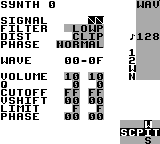
\includegraphics{synth}}
	\end{center}
	\caption{Synth Screen}
	\label{fig:synth}
\end{figure}

\subsection{General Parameters}

\begin{description}
\item[\textsc{signal}] Square, saw tooth or triangle.
\item[\textsc{filter}] Low-pass, high-pass, band-pass or all-pass.
\item[\textsc{dist}] Distortion mode. \textsc{Clip} truncates the wave to \textsc{limit}, \textsc{fold} mirrors the wave around \textsc{limit}, \textsc{wrap} wraps around vertically.
\item[\textsc{phase}] \label{phase}
Compress the waveform horizontally. It is applied after filtering with Q and cutoff. See figure \ref{fig:phasing} for examples.
\end{description}

\begin{figure}[hbtp]
	\centering
	\subfloat[Phase example. Original wave.]{
		\fbox{\includegraphics{phase-original}}
	}
	\qquad
	\subfloat[\textsc{normal} phasing. Compress horizontally, generate once.]{
	\fbox{\includegraphics{phase-normal}}
	}

	\subfloat[\textsc{resync} phasing. Compress horizontally, loop.]{
		\fbox{\includegraphics{phase-resync}}
	}
	\qquad
	\subfloat[\textsc{resyn2} phasing. Loop, but don't compress.]{
		\fbox{\includegraphics{phase-resyn2}}
	}
	\caption{Phase Examples}
	\label{fig:phasing}
\end{figure}

\subsection{Start and End Parameters}

Use these settings to specify values for the start and end of the sound. The program will then create a smooth fade between the start and end values.

\begin{description}
\item[\textsc{volume}] Signal volume.
\item[\textsc{q}] Resonance control. Boosts the signal around the cutoff frequency, to change how bright or dull the wave sounds.
\item[\textsc{cutoff}] Filter cutoff frequency.
\item[\textsc{vshift}] Shifts the signal vertically. See figure \ref{fig:vshift} for examples.
\item[\textsc{limit}] Limits the signal vertically using the \textsc{dist} mode.
\item[\textsc{phase}] 0 = no phase, \$1F = maximum phase. See figure \ref{fig:phasing} for examples.
\end{description}

\begin{figure}[htpb]
	\centering
	\subfloat[Vshift example. Original wave.]{
		\fbox{\includegraphics{vshift-original}}
	}

	\subfloat[Vshifted signal. Vshift = 40, dist = wrap.]{
	\fbox{\includegraphics{vshift-40}}
	}

	\subfloat[Vshifted signal. Vshift = 80, dist = wrap.]{
		\fbox{\includegraphics{vshift-80}}
	}
	\caption{Vshift Examples}
	\label{fig:vshift}
\end{figure}

\section{Wave Screen}
\label{wave-screen-section}

%\begin{figure}[htpb]
%	\begin{center}
%		\fbox{		\includegraphics{wave}}
%	\end{center}
%	\caption{Wave Screen}
%	\label{fig:wave}
%\end{figure}
In the wave screen, you can view and edit the individual waveforms of the synth programs. There are 16 (\$10) synth programs, and each programs has \$10 waves. This means that synth sound 0 uses waves \$0-\$F, synth sound 1 uses waves \$10-\$1F, and so on.

To change selected values, press \textsc{up/down}. To flip selected values, press \textsc{a+cursor}. \textsc{B+cursor} navigates between different waves.

It is possible to modify multiple values at once, using the regular key presses:

\begin{description}
	\item[\textsc{select+b}] Start selection.
	\item[\textsc{select+b,b}] Select the entire wave.
	\item[\textsc{b}] Copy selection to clipboard.
	\item[\textsc{up/down}] Move selection up/down.
	\item[\textsc{a+left/right}] Flip selection horizontally.
	\item[\textsc{a+up/down}] Flip selection vertically.
	\item[\textsc{select+a}] Paste from clipboard.
\end{description}

\section{Project Screen}

\begin{figure}[htpb]
	\begin{center}
		\fbox{		\includegraphics{project}}
	\end{center}
	\caption{Project Screen}
	\label{fig:project}
\end{figure}

The project screen (figure~\ref{fig:project}) contains settings that affect the entire program.

\begin{description}
	\item[\textsc{tempo}] Change the tempo. It is possible to set a new tempo either by pressing
\textsc{a+cursor}, or by tapping the \textsc{a} button up to 4 times in pace with the desired tempo. When being
slave in sync mode, it is possible to temporarily play a little faster or slower by pressing \textsc{a+left/right}.
	\item[\textsc{transpose}] Adjust the pitch of the pulse and wave instruments, by a given number of semitones.
	\item[\textsc{sync}] Activate link-up over the serial port. (Read more about this in chapter \ref{sync-chapter}!)
	\item[\textsc{clone}] Select deep or slim chain cloning. Deep chain cloning will also clone the phrases of a chain when cloning, whereas slim cloning will re-use the old phrases. Read chapter 3 for a full explanation of cloning.
	\item[\textsc{look}] Change the font and color set.
	\item[\textsc{key delay/repeat}] Set repeat delay and repeat rate of the Game Boy buttons.
	\item[\textsc{prelisten}] Play notes and instruments while entering them.
	\item[\textsc{help}] Enter help screen. The help screen contains a quick reference for button presses and a command list.
	\item[\textsc{clean song data}] Clear all phrases and chains that are not used in the song. Also, if duplicate phrases with the same content exist, they will be reduced to only one phrase. \label{clean-song-data}
	\item[\textsc{clean instr data}] Clear all instruments, tables, synths and waves that are not used in the song.
	\item[\textsc{load/save song}] Enter file manager. \footnote{The file manager is only available for cartridges that have 1 Mbit SRAM or more. In case your cartridge doesn't have 1 Mbit SRAM, this button will be replaced with a \textsc{reset memory} button.}
\end{description}

This screen also contains two clocks. The \textsc{work time} clock displays the time Little Sound Dj has been used since the last memory reset, in hours and minutes. When playing, the clock
is replaced by a \textsc{play time} clock, which shows for how long the song has been playing. The \textsc{total} clock displays the time Little Sound Dj has been used in total, in days, hours and minutes.

\subsection{Total Memory Reset}
\label{total-memory-reset}

It is possible to reset the cartridge by pressing \textsc{select+a+b} on \textsc{load/save file}. This will erase all songs and bring back the cartridge to its default state. This can be useful if memory got scrambled, or if you want to erase all songs quickly.

\section{File Screen}

\begin{figure}[htpb]
	\begin{center}
		\fbox{\includegraphics{file}}
	\end{center}
	\caption{File Screen}
	\label{fig:file}
\end{figure}

The file screen (figure~\ref{fig:file}) is entered by pressing the \textsc{load/save file} button in the project screen. The file screen is used for saving the song you are working on to the storage memory. It can also be used to load songs from the storage memory to the work memory. The file screen allows you to keep up to 32 songs on one cartridge.

\textsc{Note}: The file screen is only available for cartridges that have 1 Mbit SRAM or more.

\begin{description}
	\item[\textsc{file}] Shows the file name of the song you are working on. The exclamation mark (\textsc{!}) indicates when changes have been made to a song.
	\item[\textsc{load}] Load a song. Press \textsc{a}, select the file to load and press \textsc{a} again.
	\item[\textsc{save}] Save song. Press \textsc{a}, select the slot to save to and enter the file name.
	\item[\textsc{del}] Delete a song. Press \textsc{a}, select the file to delete and press \textsc{a} again.
	\item[\textsc{blocks used}] Shows how much of the storage memory that is used. One block equals 512 bytes. The digits on the bottom are hexadecimal, meaning there is a total of \$BF * 512 = 97,792 available bytes.
\end{description}

If you want to cancel an operation in this screen, simply press \textsc{b}.

\begin{figure}[hbtp]
\includegraphics[width=1cm]{tip}TIP!
\begin{itemize}
        \item \textit{There is a useful file manager application available at} \url{http://littlesounddj.com/lsd/latest/lsd-manager/}.
	\end{itemize}
\end{figure}

\subsection{Song List}

The song list presents song name, version number and file size. When saving, the song is compressed, so the resulting file size will vary with different songs. If you want to start a new project, load from the \textsc{(empty)} slot.

\includegraphics[width=1cm]{tip}TIP!
\begin{itemize}
    \item{While in the song list, it is possible to press \textsc{select+a} to load a song without switching to the song screen, and \textsc{start} to start/stop songs. In this way, you can load and play songs without jumping back and forth between screens. This can be handy if you are playing a live show with prepared tracks and want fewer things to think about.}
\end{itemize}

\section{Border Information}

A lot of useful data is displayed in the screen border (figure~\ref{fig:border}).

\begin{figure}[htpb]
	\begin{center}
	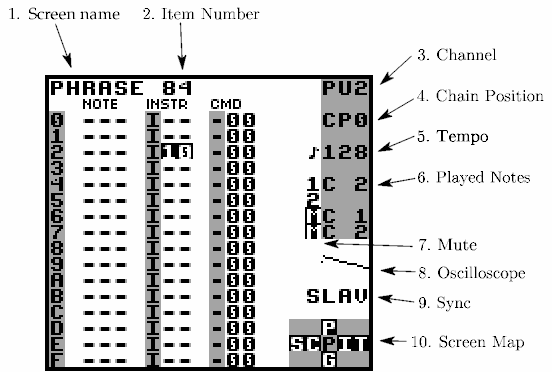
\includegraphics[width=12cm]{border}
	\end{center}
	\caption{Border Information}
	\label{fig:border}
\end{figure}

\begin{enumerate}
\item Screen name.
\item Phrase/chain/instrument/table/frame/groove number.
\item Active channel.
\item Chain position being edited.
\item Current tempo, in beats per minute (\textsc{bpm}).
\item Notes being played.
\item Sync information.
\item Mute. (Channel indicators change to \textsc{m} when pressing \textsc{b+select} or \textsc{b+start}.)
\item Oscilloscope. (The current waveform being played in the wave channel is shown.)
\item Screen map.
\end{enumerate}



\chapter{Advanced Techniques}

\section{Copy and Paste} \label{copy-paste}

Little Sound Dj has a clipboard for temporary data storage. Pressing \textsc{b+a} will cut the value
under the cursor and store it on the clipboard. The value can then be pasted by pressing
\textsc{select+a}.

In most screens, it is possible to make a selection by pressing \textsc{select+b} and moving around
the cursor. Once you have selected an area, the data can be copied to the clipboard by pressing \textsc{b},
or cut to the clipboard by pressing \textsc{select+a}. The clipboard contents can then be pasted by
pressing \textsc{select+a}.

Some quick-select button presses are implemented:
\begin{itemize}
\item \textsc{select+(b, b)} = quick-select a column or row.
\item \textsc{select+(b, b, b)} = quick-select an entire screen.
\end{itemize}

When having selected an area, you can change all data inside that selection by pressing \textsc{a+cursor}. This can be used, for example, to transpose several notes quickly.

\section{Cloning}

Cloning is a shortcut that can save you much unnecessary copy and paste action. It allows you to create copies of chains, phrases, instruments, synths, and tables directly from the song, chain, phrase and instrument screens.

Let's say you have a melody in chain 00, and you want to continue the song with the same melody, but with a slight variation. Place the cursor underneath chain 00 and press \textsc{a} once so you get:

\begin{verbatim}
 00
 00
\end{verbatim}

Now, place the cursor on the second 00, and press \textsc{select+(b, a)}.
You will now get a new chain (probably called 01) which is a copy of 00. Since it's a copy, you can play around with it as much as you want without touching 00.

\subsection{Deep vs. Slim-Cloning}

There are two different modes for cloning: slim-cloning and deep-cloning. You can select the mode in the project screen.

If you slim-clone 00, Little Sound Dj makes a new chain 01 that
contains the same phrases as 00.

If you deep-clone 00, Little Sound Dj makes a new chain 00, and
also clones the phrases within 00 into 01. That way,
you can change 01's phrases without affecting 00.

The advantage of deep-cloning is that you have no risk of modifying old phrases by accident. The drawback is that it uses more phrases, so that you may run out of phrases faster. Also, your songs may take up more blocks when being saved using the file screen.

If you find yourself running out of phrases, try using \textsc{clean song data} in project screen. (Section \ref{clean-song-data}.)

\section{The Importance of Backups}

Some words of caution from many people's hard-earned experience: If you use Little Sound Dj on a Game Boy cartridge, it is a good idea to frequently back up your songs to a PC. Some Game Boy cartridges such as the El Cheapo SD, Everdrive, or EZ Flash Junior use a microSD card which makes backup easy, but other, older Game Boy cartridges are often rather unstable, especially if they depend on an internal battery which is likely to run out sooner or later. If you are serious about your music, you should do regular backups, or at least try to record your songs once in a while.

\section{Muting, Soloing and Panning on the Fly}

It is always possible to mute a channel temporarily by pressing \textsc{b+select}. If the \textsc{b} button is released before \textsc{select}, the channel will stay muted until \textsc{b} is pressed again.

Correspondingly, a channel can be played solo by pressing \textsc{b+start}. If the \textsc{b} button is released before \textsc{start}, the other channels will stay muted. If the \textsc{start} button is released first, all channels will be turned on again.

It is also possible to pan channels left or right, by pressing \textsc{b+left/right} in the song screen.

\section{Live Mode}

 Live mode is a special flavor of the song screen. It can be activated by pressing \textsc{select+left} while in the song screen. In live mode, it is possible to start and stop playing chains one by one. In contrast to the usual song screen, the different channels can be started and stopped independently. It is also possible to jump between different song positions while playing, without causing audio glitches or going out of sync.

To play a chain, move the cursor to the chain and press \textsc{start}. To stop playing a chain, go to that channel and press \textsc{select+start}. If another chain is already playing, the starts and stops will be queued until that chain has been played through. If you want to queue until the next phrase end instead, tap \textsc{start} twice to speed up the switch.

To switch back to song mode from live mode, press \textsc{select+left} in the song screen.

\includegraphics[width=1cm]{tip}TIP!
\begin{itemize}
        \item \textit{To start or stop several chains at once, select them before pressing \textsc{start} or \textsc{select+start}. (Selecting is described in section \ref{copy-paste}.)}
	\end{itemize}

\subsection{Chain Loops}

Using chain loops is a useful live mode technique. This technique is based on the fact that the song sequencer (in live mode) won't rewind the song position all the way up to the first line of the song screen when encountering the end of the song if there is an empty line between the end of the song and the beginning; instead, the song sequencer will rewind to the empty line.

\begin{figure}[htpb]
	\begin{center}
	\fbox{\includegraphics{chainloop}}
	\end{center}
	\caption{Chain Loop Example}
	\label{fig:chainloop}
\end{figure}

Example: We have a setup that looks like figure~\ref{fig:chainloop}.

Assume that we start playing pulse channel 1 at song position 4. The player will now loop chains 2 and 3. Defining a number of such chain loops to alternate between would provide a good starting point for a live performance.

\section{Creating Synthetic Drum Instruments}

Creating good-sounding drum instruments without using the sampled drum kits might be a bit tricky, if you've had no prior experience with drum synthesis. Nevertheless, it's a very useful technique once you know it. Here are some ideas to start with:

\begin{figure}[hbtp]
	\centering
	\subfloat[Bass Drum (Pulse)]{
		\fbox{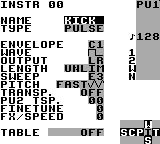
\includegraphics{instr-kick}}
	}
	\qquad
	\subfloat[Closed Hi-Hat]{
	\fbox{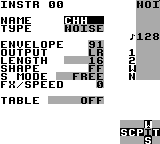
\includegraphics{instr-chh}}
	}

	\subfloat[Open Hi-Hat]{
		\fbox{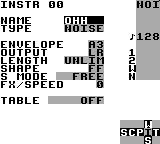
\includegraphics{instr-ohh}}
	}
	\qquad
	\subfloat[Cymbal]{
	\fbox{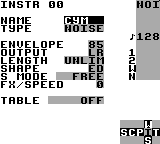
\includegraphics{instr-cym}}
	}

	\subfloat[Snare Drum]{
		\fbox{\includegraphics{instr-snare}}
	}
	\qquad
	\subfloat[Snare Drum Table]{
	\fbox{\includegraphics{table-snare}} \label{fig:table-snare}
	}

	\caption{Synthetic Drum Instruments}
	\label{fig:instr-examples}
\end{figure}

\subsection{Bass Drum (Pulse)}

You can use pulse channel 1 for creating bass drum sounds. The amplitude envelope should have a strong attack and fast decay - try setting it to \$C1. Wave should be 50-50 high/low, even though other waves can be used for making the instrument sound more distorted. The sweep value is maybe the most important part in creating a successful kick instrument. It should have a high initial frequency and decay. Try setting it to a value of \$E3, and playing the instrument at note C-4. For a more snappy sounding kick, try experimenting with the envelope and length parameters. Set \textsc{transp} to \textsc{off} to prevent transposes from changing the pitch.

\subsection{Snare Drum}

Use the noise channel for creating snare drum sounds. The amplitude envelope should have a strong attack and fast decay - try setting it to \$C1. Use the length parameter to create more snappy sounding snares. The shape parameter can be used for adjusting the timbre - shape values close to \$EC might prove useful.

\subsection{Hi-Hats and Cymbals}

Hi-hats are created using the noise channel. Use a shape value of \$FF for selecting a timbre with high frequency content. Change the envelope and length parameters for creating the desired amplitude envelope. For emulating cymbals, use a shape value near \$EE to create a somewhat rougher timbre.

\subsection{Taking Advantage of Tables}

For adding that extra punch to snares, you can use a table that uses the transpose column to change the noise shape rapidly. (See figure~\ref{fig:table-snare}.)

\begin{figure}[hbtp]
	\centering
	\subfloat[Bass Drum Instrument]{
		\fbox{\includegraphics{instr-wavekick}}
	}
	\qquad
	\subfloat[Bass Drum Synth]{
	\fbox{\includegraphics{synth-wavekick}}
	}

	\subfloat[Bass Drum Wave]{
		\fbox{\includegraphics{wave-wavekick}}
	}
	\qquad
	\subfloat[Bass Drum Table]{
	\fbox{\includegraphics{table-wavekick}}
	}

	\caption{Wave Channel Bass Drum}
	\label{fig:wavekick}
\end{figure}

\subsection{Bass Drum (Wave)}

For a more advance bass drum technique, you can make one by using the synthesizer in the wave channel. Set the \textsc{pitch} to \textsc{drum} by pressing \textsc{a+up}, and set \textsc{transp} to \textsc{off}. Set synth \textsc{play} to \textsc{manual}. On the synth screen, choose the triangle signal, and set \textsc{volume} to \$30. Set a table for the instrument. On line 0 of the table use a fast P command such as \$C0. On line 1, put \$80 in the \textsc{tsp} column and use an L command with a value such as \$30. This will transpose the bass drum to the lowest possible note without wrapping to a higher pitch.  Feel free to experiment with different synth parameters or different values for the P and L commands to shape the sound of the kick, as well as playing the instrument at note C-5, C-6, or above. (See figure~\ref{fig:wavekick}.)

\chapter{Overview of Key Presses}

This is an overview of key presses valid in the phrase screen. The key pressing philosophy expressed here is used as consistently as possible throughout the entire program.

%\section{Key Presses}

\begin{description}

\subsubsection{Editing Notes}

\item[\textsc{a}] insert note on empty step

\item[\textsc{a+right}] note up
\item[\textsc{a+left}] note down
\item[\textsc{a+up}] octave/+10 up
\item[\textsc{a+down}] octave/-10 down

\item[\textsc{b+a}] cut note to clipboard

\subsubsection{Making a Selection}
\item[\textsc{select+b}] start selecting
\item[\textsc{select+(b, b)}] select row
\item[\textsc{select+(b, b, b)}] select all

\subsubsection{When Having Made a Selection\dots}
\item[\textsc{a+left}] all selected down
\item[\textsc{a+right}] all selected up
\item[\textsc{a+up}] all selected octave/+10 up
\item[\textsc{a+down}] all selected octave/-10 down

\subsubsection{Copy/Paste Action}
\item[\textsc{b}] copy selected data to the clipboard
\item[\textsc{select+a}] cut the selected data to the clipboard

\item[\textsc{select+(b, b, b, b)}] copy the entire screen to the clipboard
\item[\textsc{select+a}] paste from the clipboard

\subsubsection{Switching Phrases}
\item[\textsc{b+left}] view the phrase in the leftmost channel
\item[\textsc{b+right}] view the phrase in the rightmost channel
\item[\textsc{b+up}] view previous phrase in chain
\item[\textsc{b+down}] view next phrase in chain

\subsubsection{Start/Stop in Song Mode}

\item[\textsc{start}] start/stop playing this phrase
\item[\textsc{select+start}] start/stop playing all channels

\subsubsection{Start/Stop in Live Mode}
\item[\textsc{start}] start playing selected chain after next chain end
\item[\textsc{start, start}] start playing selected chain after next phrase end
\item[\textsc{select+start}] stop playing current chain when it ends
\item[\textsc{select+(start, start)}] stop playing current chain after next phrase end

\subsubsection{Muting and Soloing}
\item[\textsc{b+select}] mute this channel
\item[\textsc{b+start}] solo this channel
\end{description}




\chapter{Commands}

Commands can be used in phrases and tables for altering the sound. There is a lot of power hidden in the commands, so it is suggested that you skim through this chapter at least once to get an idea of what they can do for you.

\includegraphics[width=1cm]{tip}TIP!
\begin{itemize}
        \item \textit{Tapping \textsc{a} on a command letter will display a scrolling help text in the top of the screen. \textsc{a+cursor} can then be used to browse through the existing commands. The text can be paused by holding \textsc{select}.}
	%\marginpar{\includegraphics[width=1cm]{tip}TIP!}
	\end{itemize}

\section{A: Table Start/Stop}

Starts or stops tables in the current channel. Use the table number you want to start, or 20 for stopping.

\begin{description}
\item[A03] start table 3
\item[A20] stop table
\end{description}

\section{B: mayBe}

B determines the probability that notes will play. It can also be used to probabilistically hop in a table.

\subsection{B in Phrases}

Controls how likely it is that the note or sample(s) to the left will be played. The first digit sets probability for the left kit, the second digit sets the probability for notes and right kit.

\begin{description}
    \item[B00] Never play note
    \item[B0F] Always play note/right kit sample
    \item[BF0] Always play left kit sample
	\item[B08] Play note/right kit sample about 50% of the time
\end{description}

\subsection{B in Tables}

In the table screen, B is used to make a hop that only happens sometimes. The first digit sets probability, the second digit sets destination row.

\begin{description}
\item Example:
\item[BF5] Hop to row 5, 15 times out of 16.
\item[B84] Hop to row 4, about 50% of the time.
\item[B03] Never hop to row 3
\end{description}

\section{C: Chord}

\subsection{For Pulse and Wave Instruments:}

\label{command-chord}
Produce chords by doing a simple arpeggio that extends the root note with the given semitones.

\begin{description}
\item[C37] plays a minor chord: 0, 3, 7, 0, 3, 7, 0, 3, 7, \ldots
\item[C47] plays a major chord: 0, 4, 7, 0, 4, 7, 0, 4, 7, \ldots
\item[C0C] plays 0, 0, C, 0, 0, C, 0, 0, C, \ldots
\item[CC0] plays 0, C, 0, C, 0, C, \ldots
\item[CCC] plays 0, C, C, 0, C, C, 0, C, C, \ldots
\item[C00] resets chord
\end{description}

\subsection{For Noise Instruments:}

Applies S command with the given value every second tick.

\section{D: Delay}

Delay the triggering of a note by the given number of ticks.

\section{E: Amplitude Envelope}

This command functions in two different ways, depending on which instrument type it is used on.

\subsection{For Pulse and Noise Instruments}
The first digit value sets the initial amplitude (0=min, \$F=max); the second digit sets the release (0,8: no change, 1-7: decrease, 9-\$F: increase).

\subsection{For Wave Instruments}
\begin{description}
\item[E00] volume 0\%
\item[E01] volume 25\%
\item[E02] volume 50\%
\item[E03] volume 100\%
\end{description}

\section{F: Wave Frame/Finetune}

\subsection{For Pulse Instruments:}
The first digit sets \textsc{pu2 tsp}, the second \textsc{finetune}.
See section~\ref{detune}.

\subsection{For Kit Instruments:}
Modifies the sample position. \$00-\$7F steps forward, \$80-\$FF steps back.

\subsection{For Wave Instruments:}
Change the wave frame that's being played on the wave channel. This command is relative, meaning that the command value will be added to the current frame number. This can be used for playing synth sounds manually.

\includegraphics[width=1cm]{tip}TIP!
\begin{itemize}
        \item \textit{Since a synth sound contains 16 (\$10) waves, issuing the command \textsc{F10} will in effect jump to the next synth sound.}
	%\marginpar{\includegraphics[width=1cm]{tip}TIP!}
	\end{itemize}

\begin{description}
\item Example:
\item[F01] If wave frame 3 is being played, advance 1 frame and start playing frame number 4.
\end{description}

\section{G: Groove Select}

Select the groove to use when playing phrases or tables.

\begin{description}
\item Example:
\item[G04] select groove 4
\end{description}

\section{H: Hop}

H hops to a new play position. It can also be used to stop playing.

\subsection{H in Phrases}

\begin{description}
    \item[H00-H0F] Hop to next phrase. The digit sets destination phrase step.
    \item[H10-HFE] Hop back within the phrase. The first digit sets number of times to hop back, the second digit sets destination step.
    \item[HFF] Stop playing song (or channel, if in live mode).
\end{description}

\includegraphics[width=1cm]{tip}TIP!
\nolinebreak
\begin{itemize}
        \item \textit{If you want to compose in waltz time (3/4), put \textsc{H00} commands on step \textsc{C} in every phrase.}
\end{itemize}

\subsection{H in Tables}

In the table screen, H is used for creating table loops. The first digit sets how many times the hop should be done before moving on; 0 means ``forever.'' The second digit sets the table step to jump to. Loops can be nested; that is, you can have smaller loops inside bigger ones.

\begin{description}
\item Example:
\item[H21] Hop twice to table position 1.
\item[H04] Hop to table position 4 forever.
\end{description}

\section{K: Kill Note}

\begin{description}
\item Example:
\item[K00] Kill note instantly
\item[K03] Kill note after 3 ticks
\end{description}

\section{L: Slide}

Slides to the target note in the given duration. If the instrument's \textsc{pitch} setting is \textsc{tick}, the duration is given in ticks, otherwise in n/360 seconds.

Example:

\begin{verbatim}
  C-4 ---
  F-4 L40
  --- ---
  C-4 L10
\end{verbatim}

This will result in a slide that starts with C-4, bends to F-4, and then quickly bends back to C-4.

\subsection{L in Tables}

The L command also works in the left table command column, using the transpose column to set target note relative to the root note.

\begin{figure}[htbp]
	\begin{center}
		\fbox{\includegraphics{table-slide}}
	\end{center}
	% \caption{Synth Screen}
	% \label{fig:synth}
\end{figure}

Regular transposes and slides are added together independently. In the above example, step 0 transposes one octave up. In step 1, the L command starts sliding one octave down while keeping the transpose from step 0 unchanged. In step 2, the L command is allowed to play out while the transpose stays one octave up. After some time, L will stop one octave down, cancelling out the transpose and in practice returning to the root note.

\section{M: Master Volume}

This command changes the master output volume. The first digit modifies the left output, the second digit the right. The volume can either be set with an absolute value, or changed by a relative value.

Values 0-7 are used to specify absolute volumes. Values 8-\$F give the volume a relative change; 8 is no change, 9-\$B increase, \$D-\$F decrease.

\begin{description}
\item Examples:
\item[M77] Maximize volume
\item[M08] Minimize left volume, leave right volume unchanged
\item[M99] Increase volume with 1 step
\item[MFE] Decrease left volume with 1 step, right volume with 2 steps
\end{description}

\section{O: Set Output}

Pan channel to left, right, none or both outputs.

\section{P: Pitch Bend}

\subsection{For Pulse, Wave and Kit Instruments:}

Does a pitch change with the given speed. The behavior depends on the instrument's \textsc{pitch} setting:

\begin{description}
    \item[\textsc{drum}] Logarithmic pitch bend that updates at 360 Hz. Useful for drum sounds.
	\item[\textsc{fast}] Pitch bend that updates at 360 Hz.
    \item[\textsc{tick}] Pitch bend that updates every tick. Speed can be controlled by changing \textsc{fx/speed}.
    \item[\textsc{step}] Immediate pitch change without bend.
\end{description}

Example:

\begin{description}
\item[P02] Pitch change up with speed 2.
\item[PFE] Pitch change down with speed 2. (\$FE=-2)
\end{description}

\subsection{For Noise Instruments:}

Applies S command with the given value every tick.

\section{R: Retrig the Latest Played Note}

Play the latest played note again. The first digit modulates the volume (0=no change, 1-7=increase, 8-\$F=decrease). The second digit sets a period for the retriggering, zero being the fastest and \$E the slowest. Second digit of \$F means only retrig once.

\begin{description}
\item Example:
\item[R00] very fast retriggering
\item[R0F] retrigger once
\item[RF3] medium speed retriggering, decreasing amplitude (echo effect)
\end{description}

\section{S: Sweep/Shape}

This command has different effects for different instrument types.

\subsection{Pulse Instruments}

S modulates pitch, using the Game Boy hardware. It is useful for creating bass drums and percussion. The first digit affects pitch, the second changes pitch bend velocity.

Note: S has no effect when being used in pulse channel 2!

\subsection{Kit Instruments}

S changes the loop points. The first digit modulates the offset value; the second digit modulates the loop length. (1-7=increase, 9-\$F=decrease.) Used creatively, this command can be very useful for creating a wide range of percussive and timbral effects.

\subsection{Noise Instruments}

Alters noise shape (see section~\ref{noise-instrument-parameters}).
The command is relative, meaning that the digits are independently added to the active noise shape.

\section{T: Tempo}

Change the tick frequency so that the given \textsc{tempo} will be produced (in BPM). The \textsc{tempo} setting will be accurate only if the active groove has 6 ticks per note step. If the groove has some other number of ticks per note step, the \textsc{tempo} value should be adjusted according to the formula
\begin{math}
lsdj\_bpm = (desired\_bpm \times ticks\_per\_step)/{6}
\end{math}.

Setting a value of \$00-\$27 will set the tempo to 256-295 BPM.

\begin{description}
\item Example:
\item[T80] set tempo to 128 BPM
\item[T00] set tempo to 256 BPM
\end{description}

\section{V: Vibrato}

Add vibrato. Not available for noise instruments. The vibrato speed and shape depends on the instrument's \textsc{pitch} setting.

\begin{description}
\item Example:
\item[V42] period=4, depth=2
\item[V00] reset vibrato
\end{description}

\section{W: Wave}

\subsection{For Pulse Instruments:}
Changes waveform.

\subsection{For Wave Instruments:}
The first digit sets synth sound speed, the second sets synth sound length. 0 = no change. The synth will be restarted if length is changed.

\section{Z: RandomiZe}

The Z command repeats the last non-Z command, adding a random number to the original command value. The Z value controls the maximum value of each digit to be added (each digit is added separately).

\begin{description}
\item Example:
\item[Z02] adds one of 0, 1, 2 to the original value.
\item[Z20] adds one of 0, 10, 20 to the original value.
\item[Z22] adds one of 0, 1, 2, 10, 11, 12, 20, 21, 22 to the original value.
\end{description}

Note: Randomize does not work with mayBe, Hop, Groove or Delay commands at the moment.

\chapter{Synchronization}
\label{sync-chapter}

LSDj can be synchronized with other devices, so that it is possible to run both in exactly the same tempo. You can activate synchronization by changing the \textsc{sync} mode in the project screen.

\textsc{Important}: When running synchronized, use a groove based on 6 ticks/step. Otherwise, the resulting speed might be wrong.

\section{Game Boy to Game Boy Sync}

It is possible to sync two Game Boys running LSDj with a Nintendo Game Link cable.

\subsection{Activating LSDj Sync}

Make sure that both Game Boys are turned off. Connect the Game Boys using the link cable. Now, turn on the Game Boys, and go to the project screens. Set the \textsc{sync} mode to \textsc{lsdj} on both Game Boys.

\subsection{Song Play}

When in song mode, pressing \textsc{start} starts both Game Boys from the same song position. The Game Boy on which you pressed \textsc{start} is the one that sends sync signals; this is indicated by the text \textsc{mstr} (master) appearing in the bottom right corner. The other Game Boy shows the text \textsc{slav} (slave), indicating that it is receiving sync signals.

\subsection{Live Play}

Pressing \textsc{start} in live mode makes the Game Boy start like usual; also \textsc{mstr}/\textsc{slav} texts indicate that sync signals are sent between the Game Boys. When pressing \textsc{start} on the slave Game Boy, the text \textsc{wait} appears while it is waiting for a phrase start to begin play.

\subsection{Clipboard Transfer}

When two Game Boys are linked and not playing, copying groove, chain, phrase, instr, table or synth data on one Game Boy will transfer the copied data so it can be pasted on the other Game Boy.

\subsection{Switching Master while Playing}

In some cases, it can be useful to switch which Game Boy is the master while playing. Do this by following steps:

\begin{enumerate}
    \item Set Game Boys to \textsc{lsdj} sync.
    \item Start playing.
    \item Set slave Game Boy to sync \textsc{off}.
    \item Stop master Game Boy.
    \item Set slave Game Boy to sync \textsc{lsdj}. It now becomes the master.
\end{enumerate}

\section{\textsc{Midi} Sync}

\textsc{Midi} sync requires a special \textsc{Midi} sync cable for Game Boy. For information on how to build a \textsc{Midi} to Game Boy adapter, please refer to the website at \url{http://www.littlesounddj.com}.

Usage: Plug in the sync device before turning on your Game Boy. Then, set LSDj to \textsc{Midi} slave sync mode. Pressing \textsc{start} will now make LSDj wait for and sync with any incoming \textsc{Midi} clock signals. LSDj should use grooves based on 6 ticks.

\begin{figure}[hbtp]
\includegraphics[width=1cm]{tip}TIP!
\begin{itemize}
        \item \textit{When LSDj is slave, it is possible to temporarily play
slower or faster by pressing \textsc{a+left/right} on tempo in project screen. This can
be very useful when being hooked up to some external hardware that has drifted slightly out
of sync.}
	\end{itemize}
\end{figure}

\section{Analog In}

LSDj can sync to music equipment that sends analog sync signals. This sync mode has been tested with the Korg Volca series, but works with other gear too; you can find a list at \url{http://littlesounddj.wikia.com/wiki/Analog_Sync_Compatibility}.

A cable should be easy to make, since no particular electronics are needed: all it takes is to splice a Nintendo Game Link Cable and a 3.5mm mini plug cable together. The wires should be connected as shown in the below diagram: GND goes to GND, CLK goes to CLK.

\includegraphics[clip=true,trim=0 0 460 250,angle=270,width=12cm]{analog-in}\\

As a clarification, the above diagram is looking at the cable, and the wires are probably not red and blue in reality.

Once the cable is built, connect it to the Game Boy serial port and the \textsc{sync out} of your synthesizer. In project screen, set LSDj to \textsc{analog} sync mode. The \textsc{ticks/step} setting controls how many LSDj ticks should be generated for each incoming sync signal. Depending on the synthesizer, it may be necessary to change this setting to make LSDj run at the right speed. For Korg Monotribe, it should typically be set to 6, whereas for Korg Volca, it should be C.

\section{Analog Out}

Analog Out works similar to Analog In, except that in this mode, LSDj is responsible for sending the sync signal. The cable is different than the one used for Analog In. Build it by connecting the wires as follows:

\includegraphics[clip=true,trim=0 0 460 250,angle=270,width=12cm]{analog-out}\\

As a clarification, the above diagram is looking at the cable, and the wires are probably not red and blue in reality. This cable should be connected to \textsc{sync in} of your synthesizer.

\section{Troubleshooting Cables}

When building cables, do double and triple check that the wires are connected to the right pins. You will need a multimeter for probing the pins. If they are not connected exactly like they should, you can get cables that nearly work, but the sync is a little off. The most common problem is flipped pins; remember that the diagrams are looking at the cable, not from it!

\section{Keyboard Control}

The \textsc{keybd} sync mode is not really about synchronization. Instead, it allows connecting a standard \textsc{pc} keyboard to the Game Boy, so it can be played like a piano. This is useful for live shows and improvisation. For information on how to build a \textsc{pc} keyboard to Game Boy adapter, please refer to the website at \url{http://www.littlesounddj.com}.

Important: To get a sound when playing on the keyboard, the sequencer must already be running. (Press \textsc{start} first!) The notes you play will be played back on the next step in the phrase sequencer. To get finer timing, use a faster groove for the phrase you are playing.

\subsection{Keyboard Note Layout}

\begin{figure}[htpb]
	\begin{center}
	\fbox{\includegraphics[width=12cm]{keybd-map}}
	\end{center}
	\caption{PC Keyboard Map}
	\label{fig:keybd-map}
\end{figure}

\begin{description}
\item[\textsc{space}] play using custom table
\item[\textsc{f1/f2}] octave down/up
\item[\textsc{f3/f4}] instrument down/up
\item[\textsc{f5/f6}] select custom table to assign to \textsc{space}
\item[\textsc{f8}] change pulse instrument playback channels (\textsc{PU1, PU2, PU1+2})
\item[\textsc{f9-f12}] toggle channel mute (switches on key press)
\item[\textsc{ctrl+(f9-f12)}] tap channel mute (switches on key press and release)
\item[\textsc{cursor}] move around cursor
\item[\textsc{enter}] play chain
\item[\textsc{ctrl+enter}] stop chain
\item[\textsc{page up/down}] \textsc{b+up/down}
\end{description}


\chapter{Speech Programming}
\label{speech-chapter}

\section{Introduction}

Little Sound Dj contains fifty-nine discrete speech sounds (called allophones), stored in the first four kit banks. By combining these sounds, it is possible to create any English word or phrase.

\section{Linguistics}

A few basic linguistic concepts will help you create your own library of words. First, there is no one-to-one correspondence between written letters and speech sounds; secondly, speech sounds are acoustically different depending on their position within a word.

The first problem compares to the problem that children encounter when they learn to read. Each sound in a language may be represented by more than one letter, and conversely, each letter may represent more than one sound. Because of these spelling irregularities, it is necessary to think in terms of sounds, not letters, when using allophones.

The second, and equally important, point to understand is that the acoustic signal of a speech sound may differ depending on its position within a word. For example, the initial K sound in coop will be acoustically different from the K's in keep and speak.

\section{Programming Words}

Little Sound Dj has a special speech instrument. It is locked to instrument number \$40 and can be used in the wave channel. It contains a set of 42 words, mapped out from note C-2 to note F-5.

\begin{figure}[htpb]
	\begin{center}
	\fbox{\includegraphics{speech}}
	\end{center}
	\caption{Speech Instrument Screen}
	\label{fig:speech}
\end{figure}
\begin{figure}[htpb]
	\begin{center}
	\fbox{\includegraphics{word}}
	\end{center}
	\caption{Example Word}
	\label{fig:word}
\end{figure}

		If you want to edit a word, press \textsc{select+right} to get to the word screen. It has two columns; the left column contains the allophones to be played, the right column sets duration. The word in figure~\ref{fig:word} is programmed to say "Little Sound Dj."

		In order to make things easy to remember, it is possible to rename the words by tapping A in the speech instrument screen. If you want to, it is also possible to cut and paste words in the speech instrument screen.

\section{Guidelines for Using the Allophones}

Allophones marked with * loop indefinitely.

\subsection{Short vowels}

\begin{description}
\item[*IH] sitting, stranded
\item[*EH] extent, gentlemen
\item[*AE] extract, acting
\item[*UH] cookie, full
\item[*AD] talking, song
\item[*AX] lapel, instruct
\end{description}

\subsection{Long vowels}

\begin{description}
\item[IY] treat, people, penny
\item[EY] great, statement, tray
\item[AY] kite, sky, mighty
\item[OI] noise, toy, voice
\item[UW1] after clusters with YY: computer
\item[UW2] in monosyllabic words: two, food
\item[OW] zone, close, snow
\item[AW] sound, mouse, down
\item[EL] little, angle, gentlemen
\end{description}

\subsection{R-colored vowels}

\begin{description}
\item[ER1] letter, furniture, interrupt
\item[ER2] monosyllables: bird, fern, burn
\item[OR] fortune, adorn, store
\item[AR] farm, alarm, garment
\item[YR] hear, earring, irresponsible
\item[XR] hair, declare, stare
\end{description}

\subsection{Resonants}
\begin{description}
\item[WW] we, warrant, linguist
\item[RR1] initial position: read, write, x-ray
\item[RR2] initial clusters: brown, crane, grease
\item[LL] like, hello, steel
\item[YY1] clusters: cute, beauty, computer
\item[YY2] initial position: yes, yarn, yo-yo
\end{description}

\subsection{Voiced fricatives}
\begin{description}
\item[VV] vest, prove, even
\item[DH1] word-initial position: this, then, they
\item[DH2] word-final and between vowels: bathe, bathing
\item[ZZ] zoo, phase
\item[ZH] beige, pleasure
\end{description}

\subsection{Voiceless fricatives}
\begin{description}
\item[*FF] fire, fox
\item[*TH] this, they
\item[*SS] sit, smile
\item[SH] shirt, leash, nation
\item[HH1] before front vowels: YR, IY, IH, EY, EH, XR, AE
\item[HH2] before back vowels: UW, UH, OW, OY, AO, OR, AR
\item[WH] white, whim, twenty
\end{description}

\subsection{Voiced stops}
\begin{description}
\item[BB1] final position: rib; between vowels: fibber, in clusters: bleed, brown
\item[BB2] initial position before a vowel: beast
\item[DD1] final position: played, end
\item[DD2] initial position: down; clusters: drain
\item[GG1] before high front vowels: YR, IY, IH, EY, EH, XR
\item[GG2] before high back vowels: UW, UH, OW, OY, AX; and clusters: green, glue
\item[GG3] before low vowels: AE, AW, AY, AR, AA, AO, OR, ER; and medial clusters: anger; and final position: peg
\end{description}


\subsection{Voiceless stops}
\begin{description}
\item[PP] pleasure, ample, trip
\item[TT1] final clusters before SS: tests, its
\item[TT2] all other positions: test, street
\item[KK1] before front vowels: YR, IY, IH, EY, EH, XR, AY, AE, ER, AX; initial clusters: cute, clown, scream
\item[KK2] final position: speak; final clusters: task
\item[KK3] before back vowels: UW, UH, OW, OY, OR, AR, AO; initial clusters: crane, quick, clown, scream
\end{description}

\subsection{Affricates}
\begin{description}
\item[CH] church, feature
\item[JH] judge, injure
\end{description}

\subsection{Nasal}
\begin{description}
\item[MM] milk, alarm, example
\item[NN1] before front and central vowels: YR, IY, IH, EY, EH, XR, AE, ER, AX, AW, AY, UW; final clusters: earn
\item[NN2] before back vowels: UH, OW, OY, OR, AR, AA
\end{description}




\input{kits.tex}

\end{document}

